
Testing is an integral part of every development process.
Many different testing approaches have been proposed during the history of
software development, but they all suggest that testing has to be performed continuously
during the development process. This is of particular importance to our process since
it follows an iterative approach. Testing should be planned in the early stages of each
iteration for each testable unit that is going to be implemented and performed as soon as
the iteration is complete. As the system evolves so does the testing approach which should
then be more comprehensive and cover the integration of each module into the system and the
system itself as a whole.

\section{Customer feedback}
Customer feedback was an important part of the testing approach for our project.
Working prototypes and/or documentation were produced for each meeting with the customer
in order to test the features implemented in the prototypes, receive a general acceptance
on our iteration goals and plan the next iteration. Receiving a constant feedback from the
user was very important as especially the 'social' part of the project didn't really have a
specific set of requirements from the beginning, so acquiring feedback from the customer allowed
us to understand the most common use case scenarios and from those obtain a set of requirements used
to design the system.

\section{Unit testing}
This involves testing small portions, like methods and functions, of the code, making sure they work 
as intended throughout the process of implementing code. Tests will be executed after changes in the 
code to make sure that it still works as expected, this means that unit tests have to be written for 
large portions of the API.

\section{User interface testing}
For the prototypes we made some applications that will run on an Android phone. To make sure our 
prototypes are understandable and easy to use, we have used group members that have not been 
involved in the process of making the UI, as test candidates. It might not be the ideal way of testing 
an UI, but in the given timeframe of this project it was the easiest and fastest way of doing it.

\section{Integration testing}
After each module of the API has been Unit tested, they will be put together to form bigger components 
of the working system. This is to make sure that the smaller modules will work correctly when placed 
into bigger components. 

In our case this will be to run tests on ComLib and SocialLib making sure they work individually, 
before they are tested together.

\section{System testing}
This involves butting the components from integration testing together to form a complete system that 
can be tested. Preferably each module will be added incrementaly, to easier spot wich module, if any, 
produces an error.

\section{Prototypes}
We have three different prototypes that use the oSNAP library. These three different prototypes serve
as a proof of concept and test that the library works. Each of the prototypes should have a different
application to show that the library can be used in any context and not just for one application. One of
the protoypes - the t-shirt- is significantly bigger and more complex than the other two. The t-shirt
is the prototype for the entire oSNAP library and the other two are just proof that the library works
for other applications.

\subsection{Prototype 1: The Social T-Shirt}
This is our main prototype to show the social library. A t-shirt or sweater connected to a Lilypad Arduino will have
several displays and indicator which will all receive data from the Android phone. The data sent will be social media 
statistics or updates. The shirt has many planned tangiable features (see figure \ref{fig:testing-TShirt}):
\begin{itemize}
\item LED lights
\item LCD Display
\item Sound speaker
\item Vibration module
\end{itemize}

Any of these outputs can be mapped to any model of any social network. So a "Poke" from Facebook could become a
vibration on the t-shirt. When someone "Likes" your post a small sound effect could be played, LED blinking on
status updates from Twitter, etc. The t-shirt connects to the social networks on the internet through a bluetooth
connection with an Android. This means the Android is connected to the internet and carried in the pocket of the
person using the t-shirt and is connected wirelessly with the Arduino Lilypad through Bluetooth.

\begin{figure}[h!]
\centering 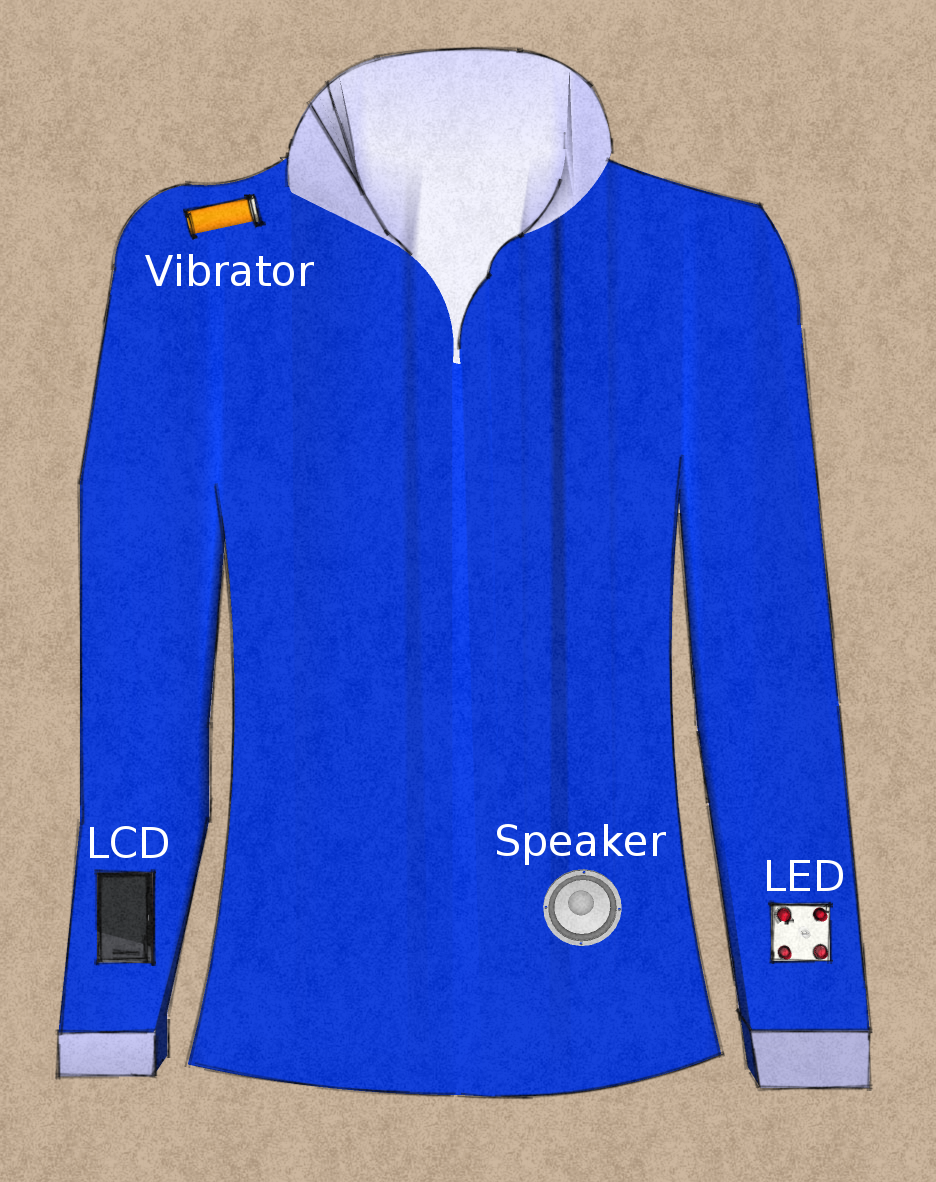
\includegraphics[scale=0.4]{img/testing-tshirtproto} \caption{Concept drawing of the T-Shirt Prototype}

\label{fig:testing-TShirt}
\end{figure}

\subsection{Prototype 2: Temperature Sensor for Android}
This prototype will primarily be made to show communication going from the Arduino to the Android over our libraries. 
A temperature sensor will be connected to an Arduino board and then constantly send it's output over bluetooth to a 
running application on Android. 

\subsection{Prototype 3: Wearable Pictures}
This prototype was first planned to be LED lights showing what mood you had on MySpace. Red LED lights would be angry,
 green would be happy and so on. We discovered that MySpace had removed this feature from their pages, however the 
support for it was still in the API available. Yet, it would be a fools errand to pursue something you could not test properly 
in a real world situation, so we changed the concept of this prototype. It ended up to be a variant of wearable fashion. 
One can take a picture or find a picture on your Android phone and choose the "Send" functionality and then choose our 
program to handle the Send. The Send is actually an intent in Android context, so it is an easy process to start our program 
from this first intent and bundle with it the picture in question. For prototyping purposes the wearable product will feature just 
a few LEDs which our Android prototype program will map to certain pixels and then transmit over Bluetooth to the Arduino 
component and this will promptly light the LEDs.
